% =============================================================================
% Lecture 6b: Network Architectures, Part 2 (Transformers and Recommenders)
% Introduction to Machine Learning Systems (Volume I)
% =============================================================================
% Attention and embedding lookups move the binding limit from arithmetic to
% memory. A four-token toy shows attention by hand; GPT-2 XL carries the costs
% of the transformer block, the quadratic score term, and decode; DLRM carries
% the recommender; the five lighthouses close the chapter in one table.
%
% Build: make -C slides build-06b_nn_architectures   (figures: images/make_figs.py)
% Plan:  lecture_map.yml and storyboard.md in this folder.
% Boundaries: Lecture 8b owns tiled attention; Lecture 13b owns LLM serving
% (batching decode, paging). This deck keeps one-line pointers to both.
% =============================================================================

\documentclass[aspectratio=169, 12pt]{beamer}
\usepackage{../../assets/beamerthememlsys}
\mlsyssetup{
  volume={Volume I},
  chapter={Chapter 6},
  chaptertitle={Network Architectures, Part 2},
  logo={../../assets/img/logo-mlsysbook.png},
  instlogo={../../assets/img/logo-harvard.png},
  layer=models,
  dividerstack,
}
\usepackage[T1]{fontenc}
\usepackage[scaled=0.9]{helvet}
\usepackage{courier}
\renewcommand{\familydefault}{\sfdefault}
\usepackage{booktabs,amsmath}
\usetikzlibrary{arrows.meta,positioning,calc}
\graphicspath{{images/}}
\setcounter{mlsystotalsections}{5}

\title{Network Architectures, Part 2}
\author{Vijay Janapa Reddi}
\institute{Harvard University}
\date{}

% A large answer choice for predict and concept-question slides
\newcommand{\choice}[2]{\textbf{\textcolor{mlsysaccent}{#1}}\enspace #2}
% A highlighted answer choice, shown from overlay #1 on
\newcommand{\answer}[3]{\alt<#1->{\colorbox{mlsysaccent!15}{\choice{#2}{#3}}}{\choice{#2}{#3}}}
% Styles for the TikZ diagrams
\tikzset{
  blk/.style={draw=#1, fill=#1!12, line width=1pt, rounded corners=2pt,
    align=center, font=\small, text=darktext, minimum height=0.8cm},
  arr/.style={-{Stealth[length=2.2mm]}, line width=0.9pt, color=midgray},
  tok/.style={inner sep=1.5pt, text=darktext, text height=1.6ex, text depth=0.3ex},
  cell/.style={draw=lightgray, line width=0.6pt, minimum width=#1, minimum height=0.55cm,
    inner sep=0pt, font=\small, text=darktext},
  cell/.default=0.6cm,
  bx/.style={draw=#1, fill=#1!10, line width=1pt, minimum width=4.0cm,
    minimum height=0.5cm, align=center, text=darktext, font=\footnotesize},
}



\begin{document}

% =============================================================================
% TITLE
% =============================================================================
\mlsysnote{[0.5 min] Read the thesis once. Say that today is the second half of the architectures chapter. Last lecture priced the families whose weights are fixed (dense, convolutional, recurrent). Today prices two bets whose memory grows with the input or exceeds the device, attention and the transformer built on it, and the recommender's embedding tables. The lecture ends by filling one table for all five lighthouse models. Notes total about 71.5 minutes. FLEX: [CORE]. Notes tagged [OPTIONAL] can be cut; cutting all of them leaves a complete lecture of about 51.5 minutes.}
\mlsystitle{Network Architectures, Part~2}{Attention and embedding tables move the limit from arithmetic to memory.}{cover_nn_architectures_blueprint.png}

% =============================================================================
% HOOK (before the first section)
% =============================================================================
\begin{frame}{Context windows grew 500 times in four years}
  \mlsysactivity{Predict}{2 min}
  \centering
  \safeimg[width=0.95\textwidth,height=4.2cm,keepaspectratio]{context_windows.pdf}\\[0.05cm]
  \uncover<2->{%
    {\normalsize 500$\times$ the window: how much more score work per layer, and memory per request?}\\[0.1cm]
    {\normalsize\choice{A}{500$\times$, 500$\times$}\qquad\choice{B}{250{,}000$\times$, 500$\times$}\qquad\choice{C}{250{,}000$\times$, 250{,}000$\times$}}}
  \mlsyscredit{Devlin et al. 2019; Radford et al. 2019; Brown et al. 2020; OpenAI DevDay, 6 Nov 2023; Anthropic, Claude 2.1, 21 Nov 2023; Google, Gemini 1.5, 15 Feb 2024 (1M in limited preview; standard 128K).}
  \note{[3 min] Step 1: the published context window, the most text a model accepts in one request, for six language models on a log scale. BERT read 512 tokens in 2018; GPT-3 read 2,048 in 2020. In November 2023 GPT-4 Turbo accepted 128,000 and Claude 2.1 200,000, and in February 2024 Google offered Gemini 1.5 Pro with up to a million tokens to a limited group of developers (its standard window was 128,000; the plot labels the point ``preview''). From GPT-3 to Gemini 1.5 the largest window grew about 500 times. Step 2: the vote. ENGAGE: students vote with one to three fingers and write one sentence on why. Do not reveal the answer; say that segment 2 answers the first number, segment 3 the second, and the last content slide prices one full request. Expected: many pick A because ``everything scales with the input''. WARN: the window states what the model accepts; this lecture computes what it costs. FLEX: [CORE].}
\end{frame}

\begin{frame}{Recall: what did recurrence cost?}
  \mlsysactivity{Retrieval}{1.5 min}
  \centering
  \only<1-2|handout:0>{%
    {\Large Close your notes.}\\[0.5cm]
    {\large A 1,000-step sequence at batch one, on 10$\times$ the FLOP/s:}\\[0.15cm]
    {\large how much faster? How much state does the RNN keep?}\\[0.6cm]
    \uncover<2->{{\Large\textbf{\textcolor{mlsysaccent}{Barely faster: 1,000 ordered steps. 2 KB of state.}}}}}%
  \only<3-|handout:1>{%
    \safeimg[width=0.92\textwidth,height=4.6cm,keepaspectratio]{state_memory.pdf}\\[0.15cm]
    {\normalsize Attention removes the serial chain and pays for it in memory.}}
  \mlsyscredit{RNN: 512-wide FP32 state (\S6.5.5). Transformer: GPT-2 XL, 307.2 KB per token in FP16 (\S6.7.4).}
  \note{[2 min] ENGAGE: thirty seconds, write both answers. Step 2: barely faster, because the 1,000 updates must run in order and each one is a batch-one matrix-vector product, limited by memory and launch overhead. The state is 2 KB, a 512-wide vector in FP32, whatever the stream length. Step 3: Part 1's plot. The blue line is the RNN's fixed state. The red line is what a transformer keeps when it generates text, 307.2 KB per token for GPT-2 XL, 3.1 GB at 10,000 tokens. Segment 3 names and sizes this store. Say the bridge aloud: ``Attention lets every token reach every other token in one step, so nothing waits in a chain. Today we price what it keeps instead.'' LINK: Part 1, recurrence segment. FLEX: [CORE].}
\end{frame}

\begin{frame}{When the bet is attention or a table, why does memory bind?}
  \begin{columns}[T]
    \begin{column}{0.36\textwidth}
      \begin{mlsyscard}{mlsysaccent}
        \textbf{Running example}\\[0.1cm]
        GPT-2 XL (Lighthouse 6.4)\\
        48 blocks, width 1,600\\
        1.5B weights\\
        3 GFLOP per token
      \end{mlsyscard}
    \end{column}
    \begin{column}{0.60\textwidth}
      \begin{itemize}\setlength{\itemsep}{0.12cm}
        \item Compute an attention head by hand, and count its work for any context.
        \item Count a transformer block's weights and FLOPs, and find where attention dominates.
        \item Explain why decode reads every weight per token, and size the KV cache.
        \item Trace a recommender's bytes, and size its tables against a device.
      \end{itemize}
    \end{column}
  \end{columns}
  \vspace{0.25cm}
  \threadstrip{0}{1}{0}{1}{1}
  \note{[1.5 min] The driving question is the title. Part 1 ended with arithmetic intensity, work per byte, compared with the machine's balance. Today's two families break that frame in two ways. A transformer adds memory that grows with the input; a recommender holds tables that may not fit at all. The card is today's running example, GPT-2 XL, 48 blocks of width 1,600, 1.5 billion weights, about 3 GFLOP per generated token. Read the four goals (what students will be able to do), one per segment; the closing table tests all four. The strip fills the algorithm factor, which attention and tables set, the machine factor, because memory now binds, and the fast-enough half. FLEX: [CORE].}
\end{frame}

% =============================================================================
% SECTION: ATTENTION
% =============================================================================
\mlsysnote{[0.5 min] Start with what attention computes, by hand, before pricing it. FLEX: [CORE].}
\mlsysdivider{What does attention compute?}{Network Architectures, \S6.6.1 to \S6.6.3, \S6.7.2, \S6.7.3}
\section{Attention}

\begin{frame}{Attention lets each token choose which tokens to read}
  \centering
  \begin{tikzpicture}[font=\normalsize]
    % Sentence 1 (chapter figure 8): weights measured in a trained BERT head
    \node[tok] (a1) at (0,0) {The};
    \foreach \w/\p/\n in {student/a1/a2, did/a2/a3, not/a3/a4, finish/a4/a5, all/a5/a6, the/a6/a7, homework/a7/a8, because/a8/a9}
      \node[tok, right=0.13cm of \p] (\n) {\w};
    \node[tok, right=0.13cm of a9, font=\normalsize\bfseries, text=BlueLine] (they) {they};
    \node[tok, right=0.13cm of they] (a11) {were};
    \node[tok, right=0.13cm of a11] (a12) {tired.};
    \draw[-{Stealth[length=3mm]}, line width=2.6pt, color=BlueLine] (they.north) to[out=160, in=20, looseness=0.55] node[pos=0.5, above, font=\small\bfseries, text=BlueLine] {0.38} (a2.north);
    \draw[-{Stealth[length=3mm]}, line width=2.1pt, color=BlueLine] (they.north) to[out=140, in=40, looseness=0.8] node[pos=0.5, above, font=\small\bfseries, text=BlueLine] {0.31} (a8.north);
    \draw[-{Stealth[length=2mm]}, line width=0.6pt, color=lightgray] (they.south) to[out=-165, in=-15, looseness=0.45] (a1.south);
    \draw[-{Stealth[length=2mm]}, line width=0.6pt, color=lightgray] (they.south) to[out=-35, in=-145, looseness=0.9] (a12.south);
    \node[anchor=west, font=\footnotesize, text=midgray] at (a12.east) {measured};
    % Sentence 2 (chapter 6.6.1)
    \uncover<2->{
    \node[tok] (b1) at (0,-2.3) {The};
    \foreach \w/\p/\n in {trophy/b1/b2, did/b2/b3, not/b3/b4, fit/b4/b5, in/b5/b6, the/b6/b7, suitcase/b7/b8, because/b8/b9}
      \node[tok, right=0.13cm of \p] (\n) {\w};
    \node[tok, right=0.13cm of b9, font=\normalsize\bfseries, text=OrangeLine] (it) {it};
    \node[tok, right=0.13cm of it] (b11) {was};
    \node[tok, right=0.13cm of b11] (b12) {too};
    \node[tok, right=0.13cm of b12, font=\normalsize\bfseries, text=OrangeLine] (b13) {\alt<3->{small.}{big.}};
    \node[anchor=west, font=\footnotesize, text=midgray] at (b13.east) {drawn};
    }
    \only<2|handout:0>{
      \draw[-{Stealth[length=3mm]}, line width=2.6pt, color=OrangeLine] (it.north) to[out=160, in=20, looseness=0.6] (b2.north);
      \draw[-{Stealth[length=2mm]}, line width=0.6pt, color=lightgray] (it.south) to[out=-150, in=-30, looseness=0.8] (b8.south);}
    \only<3-|handout:1>{
      \draw[-{Stealth[length=3mm]}, line width=2.6pt, color=OrangeLine] (it.north) to[out=145, in=35, looseness=0.8] (b8.north);
      \draw[-{Stealth[length=2mm]}, line width=0.6pt, color=lightgray] (it.south) to[out=-165, in=-15, looseness=0.5] (b2.south);}
  \end{tikzpicture}\\[0.3cm]
  \uncover<3->{\normalsize Same positions, different link, because the words decide what each token reads.}
  \mlsyscredit{Top: weights from ``they'' measured in BERT-base (uncased), layer 4, head 11; run here, images/attention\_probe.py (PyTorch 2.14.1, transformers 5.20.1). Bottom: the chapter's sentence (\S6.6.1), arrows drawn.}
  \note{[2 min] Arrow thickness is attention weight. Step 1: real weights, measured by running a trained BERT on this sentence (the script is in the images folder). From ``they'', one head puts 0.38 of its weight on ``student'' and 0.31 on ``homework'', and almost nothing on the function words, so it routes by content, to the two candidate nouns, across seven words. The head is the one of BERT's 144 that puts the most weight from ``it'' on a noun in the trophy sentence. Step 2: the chapter's trophy sentence, drawn. With ``big'', ``it'' is the trophy. Step 3: change one word to ``small'' and ``it'' is the suitcase. The positions did not change; the link did. WARN, honestly: the measured head is not this smart. It gives ``trophy'' 0.82 with ``big'' and 0.84 with ``small''; resolving the pair takes the whole model, more than any one head. A convolution's fixed window cannot route by content at all. ENGAGE: ``Give another sentence where a word's meaning depends on a word far away.'' FLEX: [OPTIONAL] If short, show step 1 only.}
\end{frame}

\begin{frame}{Attention is two matrix multiplies around a softmax}
  \centering
  \vspace{0.3cm}
  {\Large $\text{Attention}(Q,K,V) = \text{softmax}\!\left(\dfrac{\alt<2|handout:0>{\textcolor{OrangeLine}{QK^{T}}}{QK^{T}}}{\sqrt{d}}\right)\alt<4|handout:0>{\textcolor{OrangeLine}{V}}{V}$}\\[0.7cm]
  \begin{tikzpicture}[font=\normalsize]
    \uncover<2->{\node[text width=4.2cm, align=center] at (0,0) {\textbf{\textcolor{OrangeLine}{Scores}}\\$S \times S$, every pair\\$S^2 d$ multiply-adds};}
    \uncover<3->{\node[text width=4.2cm, align=center] at (4.7,0) {\textbf{\textcolor{midgray}{Softmax}}\\each row sums to 1};}
    \uncover<4->{\node[text width=4.2cm, align=center] at (9.4,0) {\textbf{\textcolor{OrangeLine}{Mix values}}\\$S^2 d$ multiply-adds\\again};}
  \end{tikzpicture}\\[0.5cm]
  \uncover<5->{\normalsize $Q$, $K$, $V$ are three learned projections of the same $S$ tokens.}
  \mlsyscredit{Network Architectures, \S6.6.2 and \S6.6.3 (Vaswani et al. 2017). $S$: sequence length; $d$: head width.}
  \note{[2 min] Step 1: the operator from the chapter. Step 2: every token's query against every token's key gives an S by S grid of scores, S squared times d multiply-adds per head. Step 3: softmax turns each row into weights that sum to one; it needs the whole row before it can finish. Step 4: the weights mix the value vectors, another S squared times d. Step 5: Q, K, and V come from three learned weight matrices applied to the same input, ordinary dense layers. The query is what a token looks for, the key what it offers, the value what it passes on. The chapter's figure 9 draws the same flow for six tokens. ENGAGE: ``Which parts grow with the square of the sequence length, and which grow linearly?'' Expected: the two products around the softmax are quadratic; the three projections are linear. FLEX: [CORE].}
\end{frame}

\begin{frame}{Four tokens through one attention head, by hand}
  \mlsysactivity{Estimate}{2 min}
  \centering
  \begin{tikzpicture}
    % headers
    \foreach \x/\t in {0.6/Q, 2.3/K, 4.0/V} \node[font=\normalsize\bfseries, text=darktext] at (\x,0.6) {$\t$};
    \node[font=\small\bfseries, text=OrangeLine] at (7.1,0.6) {scores $q_i \cdot k_j / \sqrt{2}$};
    \node[font=\small\bfseries, text=BlueLine] at (11.35,0.6) {output};
    % token numbers
    \foreach \r in {1,...,4} \node[font=\footnotesize, text=midgray] at (-0.55,-0.55*\r+0.55) {\r};
    % Q, K, V tables
    \foreach \r/\a/\b in {1/1/0, 2/0/1, 3/1/1, 4/1/0} {
      \node[cell] at (0.3,-0.55*\r+0.55) {\a}; \node[cell] at (0.9,-0.55*\r+0.55) {\b};}
    \foreach \r/\a/\b in {1/2/0, 2/0/2, 3/1/1, 4/0/0} {
      \node[cell] at (2.0,-0.55*\r+0.55) {\a}; \node[cell] at (2.6,-0.55*\r+0.55) {\b};}
    \foreach \r/\a/\b in {1/1/0, 2/0/1, 3/1/1, 4/0/0} {
      \node[cell] at (3.7,-0.55*\r+0.55) {\a}; \node[cell] at (4.3,-0.55*\r+0.55) {\b};}
    % score grid outline and key labels
    \foreach \c in {1,...,4} {
      \node[font=\footnotesize, text=midgray] at (5.1+\c,-2.35) {$k_{\c}$};
      \foreach \r in {1,...,4} \node[cell=1.0cm] at (5.1+\c,-0.55*\r+0.55) {};}
    % output grid outline
    \foreach \r in {1,...,4} {\node[cell=0.9cm] at (10.9,-0.55*\r+0.55) {}; \node[cell=0.9cm] at (11.8,-0.55*\r+0.55) {};}
    % step 2: row 1 scores
    \only<2-|handout:1>{
      \foreach \c/\v in {1/1.41, 2/0, 3/0.71, 4/0}
        \node[cell=1.0cm, fill=OrangeL] at (5.1+\c,0) {\v};}
    % step 3: softmax of row 1
    \only<3-|handout:1>{
      \node[font=\footnotesize, text=midgray, anchor=east] at (5.55,-2.95) {softmax, row 1};
      \foreach \c/\v in {1/0.51, 2/0.12, 3/0.25, 4/0.12}
        \node[cell=1.0cm, fill=BlueL, font=\small\bfseries] at (5.1+\c,-2.95) {\v};}
    % step 4: output row 1
    \only<4-|handout:1>{
      \node[cell=0.9cm, fill=BlueL, font=\small\bfseries] at (10.9,0) {0.75};
      \node[cell=0.9cm, fill=BlueL, font=\small\bfseries] at (11.8,0) {0.37};}
    % step 5: row 2 for the students
    \only<5|handout:0>{
      \foreach \c in {1,...,4} \node[cell=1.0cm, fill=mlsysaccent!12, font=\small\bfseries, text=mlsysaccent] at (5.1+\c,-0.55) {?};
      \node[cell=0.9cm, fill=mlsysaccent!12, font=\small\bfseries, text=mlsysaccent] at (10.9,-0.55) {?};
      \node[cell=0.9cm, fill=mlsysaccent!12, font=\small\bfseries, text=mlsysaccent] at (11.8,-0.55) {?};}
    % step 6: everything
    \only<6-|handout:1>{
      \foreach \r/\a/\b/\c/\d in {2/0/1.41/0.71/0, 3/1.41/1.41/1.41/0, 4/1.41/0/0.71/0} {
        \node[cell=1.0cm] at (6.1,-0.55*\r+0.55) {\a}; \node[cell=1.0cm] at (7.1,-0.55*\r+0.55) {\b};
        \node[cell=1.0cm] at (8.1,-0.55*\r+0.55) {\c}; \node[cell=1.0cm] at (9.1,-0.55*\r+0.55) {\d};}
      \foreach \r/\a/\b in {2/0.37/0.75, 3/0.62/0.62, 4/0.75/0.37} {
        \node[cell=0.9cm, font=\small\bfseries] at (10.9,-0.55*\r+0.55) {\a};
        \node[cell=0.9cm, font=\small\bfseries] at (11.8,-0.55*\r+0.55) {\b};}
      \draw[RedLine, line width=1.2pt, rounded corners=2pt] (10.4,0.3) rectangle (12.3,-0.3);
      \draw[RedLine, line width=1.2pt, rounded corners=2pt] (10.4,-1.35) rectangle (12.3,-1.95);}
  \end{tikzpicture}\\[0.25cm]
  \normalsize
  \only<1|handout:0>{Four tokens, width $d = 2$. Each output row is a weighted mix of the rows of $V$.}%
  \only<2|handout:0>{Row 1: $q_1 = (1,0)$ against each key, divided by $\sqrt{2}$.}%
  \only<3|handout:0>{Softmax turns row 1 into weights that sum to 1.}%
  \only<4|handout:0>{Output 1 $= 0.51\,v_1 + 0.12\,v_2 + 0.25\,v_3 + 0.12\,v_4 = (0.75, 0.37)$.}%
  \only<5|handout:0>{\textbf{Your turn, in pairs:} row 2's scores, weights, and output.}%
  \only<6-|handout:1>{Equal queries (1 and 4) read the same mix. Work: $4^2 \times 2 = 32$ MACs, twice: $S^2 d$ each.}
  \mlsyscredit{Illustrative toy, values computed in images/make\_figs.py. Operator: Network Architectures, \S6.6.2.}
  \note{[5 min] [CORE] Worked example 1, by hand. The numbers are a toy chosen for easy arithmetic, and no model learned them. Step 1: four tokens, each with a query, key, and value of width two. Step 2: token 1's query (1, 0) against each key gives 2, 0, 1, 0; divided by the square root of 2: 1.41, 0, 0.71, 0. Two design points live here. Queries and keys come from different weight matrices, so ``1 looks at 3'' need not score like ``3 looks at 1''. The divisor keeps the scores' variance near one as the head widens, so softmax does not saturate. Step 3: softmax of row 1: 0.51, 0.12, 0.25, 0.12. Step 4: those weights mix the value rows into (0.75, 0.37). Step 5: ENGAGE, two minutes in pairs on row 2. Expected: scores 0, 1.41, 0.71, 0; weights 0.12, 0.51, 0.25, 0.12; output (0.37, 0.75), the mirror of row 1. Step 6: rows 1 and 4 share a query and read the same mix, whatever their positions, because attention routes by content. Token 3 spreads its weight about 0.31 over tokens 1 to 3. Work: 32 multiply-adds for the scores and 32 for the mix, S squared times d each. WARN: students who skip the softmax use raw scores as weights.}
\end{frame}

\begin{frame}{Twelve heads of 64 cost the same as one head of 768}
  \centering
  \begin{tikzpicture}[font=\small]
    \node[draw=midgray, fill=vlightgray!60, minimum width=1.0cm, minimum height=1.5cm] (E) at (0,0) {};
    \node[above=0.1cm of E, text=darktext] {Tokens};
    \node[below=0.1cm of E, text=midgray, align=center] {6 $\times$ 768};
    \node[font=\Large] at (1.05,0) {$\times$};
    \foreach \x/\l/\c in {2.4/Q/BlueLine, 3.7/K/RedLine, 5.0/V/GreenLine}
      \node[draw=\c, fill=\c!15, minimum width=1.3cm, minimum height=2.2cm, font=\large\bfseries, text=\c] at (\x,0) {\l};
    \node[above=1.2cm, text=darktext] at (3.7,0) {Packed weights};
    \node[below=1.2cm, text=midgray] at (3.7,0) {768 $\times$ 2,304};
    \node[font=\Large] at (6.25,0) {$=$};
    \foreach \x/\l/\c in {7.5/Q/BlueLine, 8.8/K/RedLine, 10.1/V/GreenLine}
      \node[draw=\c, fill=\c!15, minimum width=1.3cm, minimum height=1.5cm, font=\large\bfseries, text=\c] (o\l) at (\x,0) {\l};
    \node[above=0.85cm, text=darktext] at (8.8,0) {Q, K, V for all six tokens};
    \node[below=0.85cm, text=midgray] at (8.8,0) {6 $\times$ 2,304, one kernel};
    \uncover<2->{
      \foreach \x in {6.85,9.45} \foreach \i in {1,...,11} \draw[white, line width=0.9pt] (\x+0.1083*\i,0.74) -- (\x+0.1083*\i,-0.74);
      \foreach \i in {1,...,11} \draw[white, line width=0.9pt] (8.15+0.1083*\i,0.74) -- (8.15+0.1083*\i,-0.74);
      \foreach \x/\l/\c in {7.5/Q/BlueLine, 8.8/K/RedLine, 10.1/V/GreenLine}
        \node[fill=\c!15, inner sep=1.5pt, font=\large\bfseries, text=\c] at (\x,0) {\l};
      \node[text=BlueLine, font=\normalsize\bfseries, align=left, anchor=west] at (11.1,0) {12 heads\\of 64 each};}
  \end{tikzpicture}\\[0.5cm]
  \uncover<2->{\normalsize Head widths sum to 768: the same multiply-adds, split 12 ways.}
  \mlsyscredit{After the chapter's QKV projection figure (\S6.6.2, figure 10). GPT-2 Small: width 768, 12 heads (MLSysIM GPT2\_Small).}
  \note{[1.5 min] GPT-2 Small, the chapter's figure 10. Step 1: six tokens, each a 768-wide vector, multiply one packed weight matrix that holds the query, key, and value weights side by side, 768 by 2,304. One kernel produces all three projections, which keeps the accelerator's matrix units busy and saves two kernel launches. Step 2: each 768-wide projection is cut into 12 heads of 64. Each head runs its own attention, and their outputs are concatenated and projected back to 768. ENGAGE: ``Twelve heads: twelve times the score work?'' Expected: no. Each head does S squared times 64, and 12 of them do S squared times 768, the same as one wide head. Heads buy different patterns at the same arithmetic; analyses of BERT find heads that specialize and heads that are redundant (Clark et al. 2019). WARN: the cache on later slides is sized by the key and value widths, so head count matters there. FLEX: [OPTIONAL] Say the last sentence aloud on the next slide.}
\end{frame}

\begin{frame}[fragile]{In real code, attention is one packed projection and two products}
  \vspace{-0.4cm}
\begin{semiverbatim}\footnotesize
\textcolor{GreenLine}{self.c_attn = nn.Linear(config.n_embd, 3 * config.n_embd, ...)}
\textcolor{GreenLine}{self.c_proj = nn.Linear(config.n_embd, config.n_embd, ...)}
\textcolor{midgray}{...}
q, k, v  = self.c_attn(x).split(self.n_embd, dim=2)
\textcolor{midgray}{...}
\textcolor{OrangeLine}{att = (q @ k.transpose(-2, -1)) * (1.0 / math.sqrt(k.size(-1)))}
att = att.masked_fill(self.bias[:,:,:T,:T] == 0, float(\textquotesingle-inf\textquotesingle))
att = F.softmax(att, dim=-1)
\textcolor{midgray}{...}
\textcolor{OrangeLine}{y = att @ v}
\end{semiverbatim}
  \vspace{-0.2cm}
  \centering\small
  \uncover<2->{\textcolor{GreenLine}{\textbf{Green:}} the $4d^2$ weights.\quad
  \textcolor{OrangeLine}{\textbf{Orange:}} the two $S^2 d$ products.}
  \uncover<3->{Both lower onto matrix multiplies.}
  \mlsyscredit{nanoGPT model.py, class CausalSelfAttention, lines 35 to 69 (github.com/karpathy/nanoGPT, commit 3adf61e, MIT). ``...'' marks omitted lines and the argument bias=config.bias; indentation and comments removed.}
  \note{[2 min] [OPTIONAL] Real code from nanoGPT, a few hundred lines that load the published GPT-2 weights. Step 1: read it top down; the first two lines are from the constructor, the rest from forward. c\_attn is the packed projection from two slides back, one d by 3d matrix; split cuts its output into Q, K, and V, and the omitted lines reshape each into n\_head heads of width C over n\_head. Then read the equation line by line, q times k transposed, scaled by one over the square root of the head width; the causal mask sets later positions to minus infinity; softmax; att times v. Step 2: the green lines are the weights, 3 d squared plus d squared, 4 d squared. The orange lines are the two products whose cost grows with S squared; neither holds a weight. Step 3: every colored line is a matrix multiply, which is how a GPU runs attention; the softmax and mask are element-wise passes. ENGAGE: ``Which line would you change for grouped-query attention?'' Expected: the projection, so K and V get fewer heads than Q. WARN: on PyTorch 2 nanoGPT calls one fused kernel instead of these four lines (Lecture 8b); the arithmetic is the same. FLEX: cut freely.}
\end{frame}

\begin{frame}[fragile]{A transformer block pairs attention and an MLP, each with a skip}
  \begin{columns}[c]
    \begin{column}{0.42\textwidth}
      \centering
      \begin{tikzpicture}[font=\small]
        \node[bx=RedLine] (emb) at (0,0) {Token embedding + position};
        \node[bx=GreenLine] (att) at (0,1.0) {Masked multi-head attention};
        \node[bx=BrownLine] (n1) at (0,1.75) {Add \& Norm};
        \node[bx=BlueLine] (ff) at (0,2.65) {Feed forward};
        \node[bx=BrownLine] (n2) at (0,3.4) {Add \& Norm};
        \node[bx=OrangeLine] (out) at (0,4.4) {Linear + softmax};
        \draw[arr] (emb) -- (att); \draw[arr] (att) -- (n1); \draw[arr] (n1) -- (ff); \draw[arr] (ff) -- (n2); \draw[arr] (n2) -- (out);
        \draw[arr] (0,0.5) -- (2.35,0.5) -- (2.35,1.75) -- (n1.east);
        \draw[arr] (0,2.15) -- (2.35,2.15) -- (2.35,3.4) -- (n2.east);
        \draw[lightgray, line width=0.8pt, dashed, rounded corners=3pt] (-2.3,0.6) rectangle (2.6,3.8);
        \node[font=\small\bfseries, text=midgray, anchor=east] at (-2.35,2.2) {$\times 48$};
      \end{tikzpicture}
    \end{column}
    \begin{column}{0.54\textwidth}
      \normalsize
      \uncover<2->{\textcolor{GreenLine}{\textbf{Attention:}} $4d^2$ weights\\{\small Q, K, V, and output projections}\\[0.35cm]}
      \uncover<2->{\textcolor{BlueLine}{\textbf{Feed forward:}} $8d^2$ weights\\{\small $d \rightarrow 4d \rightarrow d$}\\[0.35cm]}
      \begin{uncoverenv}<3->\textcolor{BrownLine}{\textbf{Add \& Norm:}} Part 1's skips, in nanoGPT:
\begin{semiverbatim}\footnotesize
x = x + self.attn(self.ln_1(x))
x = x + self.mlp(self.ln_2(x))
\end{semiverbatim}
      \end{uncoverenv}
      \uncover<3->{{\large\textbf{\textcolor{mlsysaccent}{$12d^2$ weights per block}}}}
    \end{column}
  \end{columns}
  \mlsyscredit{Decoder tower after the chapter's transformer figure (\S6.7.2, figure 11). Counts: Table 7, feed-forward width $4d$. Code: nanoGPT model.py, Block.forward, lines 104 and 105 (commit 3adf61e, MIT).}
  \note{[1.5 min] A decoder-only model such as GPT-2 keeps only the right-hand tower of the chapter's figure 11, without the attention that reads an encoder. Step 1: tokens enter as embedding vectors plus a position signal (sinusoidal in the original paper, rotary in many newer models; position costs little next to what follows). Inside each of the 48 blocks, masked multi-head attention mixes information across positions, and a two-layer feed-forward network transforms each position on its own. Step 2: the weight count. The four projections are d by d each, 4 d squared. The feed-forward network goes from d to 4d and back, 8 d squared. Step 3: the Add and Norm boxes are Part 1's skip connections and layer normalization, reused; the gray arrows are the skips, and nanoGPT's Block.forward is exactly these two lines: normalize, transform, add back the input. The block holds 12 d squared weights, and nothing in it depends on the context length. ENGAGE: ``Where are the attention scores in this weight count?'' Expected: nowhere; scores are computed and never stored. WARN: GPT-2 normalizes before each sublayer, as the code shows; the drawing puts it after; newer decoders change more (RMSNorm, gated MLPs, shared key-value heads), so 12 d squared is a counting rule for the classic block. LINK: Part 1, depth segment. FLEX: [CORE].}
\end{frame}

\begin{frame}[fragile,t]{GPT-2 XL's 1.5B weights follow from one rule}
  \mlsysactivity{Estimate}{2.5 min}
  \vspace{-0.6cm}
  \begin{columns}[T]
    \begin{column}{0.33\textwidth}
\begin{semiverbatim}\footnotesize
"n_embd": 1600,
"n_head": 25,
"n_layer": 48,
"vocab_size": 50257
\end{semiverbatim}
    \end{column}
    \begin{column}{0.63\textwidth}
      \small
      \uncover<2->{$12 \times 1{,}600^2 = 30.7$M per block\\[0.05cm]
      $\times\,48 =$ \textbf{1.47B}; $+$ 80M token table $\approx$ \textbf{1.55B}\\[0.2cm]}
      \uncover<4->{FLOPs per token $\approx 2 \times 1.47$B $=$ \textbf{2.95 GFLOP} (chapter: 3)}
    \end{column}
  \end{columns}
  \vspace{-0.1cm}
  \centering
  \uncover<3->{\safeimg[width=0.95\textwidth,height=2.8cm,keepaspectratio]{gpt2xl_params.pdf}}
  \mlsyscredit{Left: config.json of huggingface.co/openai-community/gpt2-xl (revision 15ea56d), four of its fields. Block rule: Table 7; values: images/calcs.py.}
  \note{[3.5 min] Worked example 2. Left: four lines of the model's real configuration file, the one that loading GPT-2 XL reads; every input below comes from it. ENGAGE: two minutes in pairs on the weights, then reveal. Step 2: 12 times 1,600 squared is 30.7 million weights per block; times 48 blocks, 1.47 billion. The token table, one 1,600-wide row for each of 50,257 tokens, adds 80 million, about 1.55 billion in all. Step 3: the bar. Attention projections 0.49 billion, the MLPs 0.98 billion, the token table 0.08 billion, against the published 1.5 billion. Counting the biases, norms, and 1,024 position rows as well gives 1,558 million, the figure nanoGPT's source prints for gpt2-xl. Two thirds of a transformer's weights sit in its MLPs. Step 4: each weight takes part in one multiply-add per token, two FLOPs, so about 2.95 GFLOP per token, the chapter's 3 GFLOP. Say the landing line: ``The scores add arithmetic but no weights.'' The next slide prices that arithmetic. WARN: students multiply 1.5 billion by 4 bytes and call it the decode traffic; that is right for FP32 and doubles the FP16 figure, so ask which precision. FLEX: [CORE].}
\end{frame}

% =============================================================================
% SECTION: QUADRATIC
% =============================================================================
\mlsysnote{[0.5 min] The hook asked about score work. Now count it. FLEX: [CORE].}
\mlsysdivider{What does letting every token see every other token cost?}{Network Architectures, \S6.6.4 and \S6.7.4 (Training and prefill)}
\section{Quadratic}

\begin{frame}{Predict: how much of a block's work is attention?}
  \mlsysactivity{Predict}{1.5 min}
  \centering
  {\large GPT-2 XL, one block, a 1,024-token prompt.}\\[0.15cm]
  {\large What share of its multiply-adds are the two attention products?}\\[0.3cm]
  \begin{minipage}{0.5\textwidth}
    \Large
    \choice{A}{About 90 percent}\\[0.15cm]
    \choice{B}{About 50 percent}\\[0.15cm]
    \answer{2}{C}{About 10 percent}
  \end{minipage}\\[0.3cm]
  \uncover<2->{\normalsize 3.36B of 34.8B MACs. The quadratic term is still small here.\\[0.1cm]
  {\small Whole prompt: $1{,}024 \times 2.95$ GFLOP $=$ 3.02 TFLOP, $+$ 0.32 attention $=$ 3.34 TFLOP}}
  \mlsyscredit{Derived from the block account, \S6.7.3 and \S6.7.4: $12Sd^2$ against $2S^2d$, $d = 1{,}600$.}
  \note{[2 min] [OPTIONAL] ENGAGE: vote with fingers. Many will pick A, because ``attention is quadratic'' sounds like ``attention is most of the work''. Step 2: C. Per block, the projections and MLP cost 12 S d squared, 31.5 billion multiply-adds at 1,024 tokens; the two attention products cost 2 S squared d, 3.36 billion. About 10 percent. The last line prices the whole prompt. 1,024 tokens times the 2.95 GFLOP of weight work per token is 3.02 TFLOP; the attention products over all 48 blocks add 0.32 TFLOP (3.36 billion multiply-adds, two FLOPs each, times 48); 3.34 TFLOP in all. WARN: quadratic describes how a cost grows and says nothing about how large it is today; a quadratic term with a small coefficient can stay behind a linear one for a long way. FLEX: if cut, give the 10 percent share on the next slide.}
\end{frame}

\begin{frame}{Attention's products overtake the rest only past 9,600 tokens}
  \centering
  \mlsyssteps[width=0.95\textwidth,height=5.0cm,keepaspectratio]{block_macs_step}{4}\\[0.1cm]
  \uncover<4->{\normalsize Short contexts are bound by ordinary dense multiplies.}
  \mlsyscredit{Derived from the chapter's block account (\S6.7.3); crossover at $6d$ (\S6.7.4). GPT-2 XL, $d = 1{,}600$ (MLSysIM).}
  \note{[2.5 min] Explain the axes first, context length across multiply-adds per block up, both on log scales, so a straight line's slope is its power. Step 1: the orange line, projections and MLP, grows in proportion to S (slope one). The blue line, the two attention products, grows with S squared (slope two). Step 2: at 1,024 tokens the gap is about ten to one, the vote's answer. Step 3: the lines cross where 12 S d squared equals 2 S squared d, at S equal to 6 d, 9,600 tokens for GPT-2 XL, as the chapter states. Step 4: at 100,000 tokens attention is about ten times everything else. ENGAGE: ``A model twice as wide: where is the crossover?'' Expected: twice as far out, because the crossover is 6 d. WARN: this counts arithmetic only. Storing the scores is a separate cost, and it is the next slide. FLEX: [CORE].}
\end{frame}

\begin{frame}{100,000 tokens would need 240 GB of scores per layer}
  \begin{columns}[c]
    \begin{column}{0.44\textwidth}
      \centering\safeimg[width=\textwidth,height=4.9cm,keepaspectratio]{quadratic.pdf}
    \end{column}
    \begin{column}{0.54\textwidth}
      \normalsize
      \textbf{Given:} a 12-head, 32-layer model (not GPT-2 XL), 100,000 tokens, FP16 scores\\[0.3cm]
      \uncover<2->{$100{,}000^2 \times 12 = 1.2 \times 10^{11}$ scores\\[0.3cm]}
      \uncover<3->{$\times$ 2 bytes $=$ {\Large\textbf{\textcolor{mlsysaccent}{240 GB}}} per layer\\[0.3cm]}
      \uncover<4->{32 layers kept for training: 7,680 GB}
    \end{column}
  \end{columns}
  \mlsyscredit{Network Architectures, Definition 6.5 and Napkin Math 6.1. Plot: one layer's scores, 12 heads, FP16.}
  \note{[2.5 min] Worked example 3 uses the chapter's generic 12-head, 32-layer model in place of GPT-2 XL. Step 1, the plot, stores one layer's scores for 12 heads in FP16. At 4,096 tokens that is 0.40 GB; at 8,192 it is 1.61 GB, four times as much for twice the tokens. ENGAGE: one minute in pairs on the given before step 2. Step 2: 100,000 squared is 10 to the 10th; times 12 heads, 1.2 times 10 to the 11th scores. Step 3: two bytes each, 240 GB for one layer, three times an 80 GB accelerator. Step 4: training that kept every layer's scores for the backward pass would need 7,680 GB. Students who get 2.4 GB dropped a factor of 100 in the square. LINK: Lecture 8b shows how tiling avoids storing the scores. FLEX: [CORE].}
\end{frame}

\begin{frame}[t]{True or false? Two claims about attention's cost}
  \mlsysactivity{Vote}{1.5 min}
  \vspace{-0.2cm}
  {\small
  \begin{tabular}{@{}l@{}}
    \textbf{1.} BERT could read 4,096 tokens on an accelerator with enough memory.\\
    \uncover<2->{\textbf{\textcolor{mlsysaccent}{False.}} It learned 512 positions; and 4,096 tokens need 64$\times$ the score memory.}\\[0.15cm]
    \textbf{2.} A tiled kernel that never stores the scores makes attention's work grow linearly.\\
    \uncover<2->{\textbf{\textcolor{mlsysaccent}{False.}} Tiling removes the $S^2$ storage; the $S^2$ multiply-adds remain.}
  \end{tabular}}\\[0.15cm]
  \centering
  \uncover<3->{\safeimg[width=14.2cm]{flash_measured.pdf}}
  \mlsyscredit{Network Architectures, Example 6.4 (Devlin et al. 2019) and \S6.6.4. Plot: Dao et al., NeurIPS 2022, Tables 20 and 21 (A100, batch 16, 8 heads of 64, FP16).}
  \note{[2.5 min] [OPTIONAL] ENGAGE: thumbs up or down for each claim, then reveal. Claim 1: false for two reasons. BERT was pretrained with 512 learned position embeddings, so positions beyond 512 do not exist for the model, however much memory there is. And cost set part of the limit, because 4,096 tokens would need (4,096 over 512) squared, 64 times the score memory. Claim 2: false. A tiled kernel streams blocks of scores through on-chip memory and never writes the full S by S matrix, so the quadratic storage goes away; every one of the S squared scores is still computed, so the quadratic arithmetic stays (section 6.6.4). Step 3: the measurement, from the FlashAttention paper's tables on an A100. Right: the tiled kernel's memory doubles when the sequence doubles, 0.84 GB at 4K and 13.4 GB at 64K, while standard PyTorch attention needs 20 times more at 4K and then runs out. Left: the tiled kernel's runtime still grows four times per doubling (3,272 times from 1K to 64K, against 4,096 for a pure square). Landing line for the segment: ``Score work grows with the square of the context; it dominates only past about six times the model width, and storing the scores would not fit long before that.'' FLEX: if cut, say the land line earlier.}
\end{frame}

% =============================================================================
% SECTION: DECODE
% =============================================================================
\mlsysnote{[0.5 min] The hook's second number is memory per request. It comes from generating text one token at a time. FLEX: [CORE].}
\mlsysdivider{Why does generating text wait on memory?}{Network Architectures, \S6.7.2 and \S6.7.4}
\section{Decode}

\begin{frame}{One model runs a prompt in parallel and a reply one token at a time}
  \centering
  \begin{tikzpicture}[font=\footnotesize]
    % Step 1: the causal mask on the prompt
    \foreach \w/\i in {The/1, cat/2, sat/3, on/4} {
      \node[anchor=east, text=darktext] at (-0.05,2.3-0.42*\i) {\w};
      \node[rotate=60, anchor=south west, text=darktext] at (0.42*\i-0.5,2.15) {\w};}
    \foreach \r in {1,...,4} \foreach \c in {1,...,4} {
      \ifnum\c>\r
        \node[draw=white, fill=vlightgray, minimum size=0.42cm, inner sep=0pt] at (0.42*\c-0.21,2.3-0.42*\r) {};
      \else
        \node[draw=white, fill=OrangeLine!45, minimum size=0.42cm, inner sep=0pt] at (0.42*\c-0.21,2.3-0.42*\r) {};
      \fi}
    \node[text width=2.9cm, align=center, text=darktext, anchor=north] at (0.5,0.1) {Causal mask: each token sees itself and earlier tokens};
    % Step 2: prefill writes the KV cache
    \uncover<2->{
      \node[font=\small\bfseries, text=OrangeLine] at (4.1,2.75) {Prefill: compute bound};
      \foreach \i/\w in {0/The,1/cat,2/sat,3/on}
        \node[blk=midgray, font=\footnotesize, minimum width=0.8cm, minimum height=0.55cm] (p\i) at (2.75+0.9*\i,1.95) {\w};
      \node[blk=OrangeLine, minimum width=3.6cm, minimum height=0.9cm] (pp) at (4.1,0.7) {One pass, all prompt\\tokens: matrix $\times$ matrix};
      \foreach \i in {0,...,3} \draw[arr] (p\i) -- (p\i |- pp.north);
      \node[draw=VioletLine, fill=VioletLine!10, line width=1pt, rounded corners=2pt, minimum height=0.6cm,
        minimum width=10.25cm, anchor=west, text=darktext, font=\footnotesize] (kv) at (2.3,-0.75)
        {\textbf{KV cache:} the keys and values of every token so far};
      \draw[arr, color=OrangeLine] (pp.south) -- (pp.south |- kv.north) node[pos=0.45, right, font=\scriptsize, text=OrangeLine] {writes};}
    % Step 3: decode, one token per step, each step reading the whole cache
    \uncover<3->{
      \node[font=\small\bfseries, text=BlueLine] at (9.6,2.75) {Decode: memory bound};
      \foreach \i/\w in {0/the,1/mat,2/end} {
        \node[blk=BlueLine, minimum width=1.45cm, minimum height=0.9cm] (d\i) at (7.4+2.2*\i,0.7) {matrix $\times$\\vector};
        \node[font=\small\bfseries, text=darktext] (o\i) at (7.4+2.2*\i,1.95) {\w};
        \draw[arr] (d\i.north) -- (o\i.south);
        \draw[{Stealth[length=2mm]}-{Stealth[length=2mm]}, line width=0.9pt, color=VioletLine] (d\i.south) -- (d\i.south |- kv.north);}
      \draw[arr] (pp.east) -- (d0.west);
      \draw[arr] (d0) -- (d1); \draw[arr] (d1) -- (d2);}
  \end{tikzpicture}\\[0.35cm]
  \uncover<3->{\normalsize The same weights are compute bound in prefill and memory bound in decode.}
  \mlsyscredit{After the chapter's prefill and decode figure, \S6.7.2 (figure 12). Mask: \S6.7.2.}
  \note{[2.5 min] Step 1: the causal mask on a four-token prompt. Rows are queries, columns are keys. The gray cells, later tokens, get a score of minus infinity before the softmax, so each token reads only itself and what came before, exactly what will exist when the model generates. Step 2, prefill: the whole prompt goes through the model in one pass as matrix-matrix products; each weight is reused across every prompt token, so prefill is usually compute bound. As it goes, it writes each token's keys and values, for every layer, into a store called the KV cache, the purple bar. The next slides draw and size it. Step 3, decode: the reply comes one token per step, and each emitted token (``the'', then ``mat'') is the next step's input. Each step multiplies the weights by one vector, reads the whole cache (the purple arrows), and appends one token's keys and values. ENGAGE: ``Why can decode not run its tokens in parallel the way prefill does?'' Expected: token t is not known until step t minus 1 finishes. WARN: the chapter's fallacy, ``an architecture has one bottleneck''. The same weights are compute bound in one phase and memory bound in the other. FLEX: [CORE].}
\end{frame}

\begin{frame}{Your turn: how fast can a 70B model write one reply?}
  \mlsysactivity{Estimate}{2.5 min}
  \begin{columns}[T]
    \begin{column}{0.60\textwidth}
      \centering
      \safeimg[width=\textwidth]{decode_ridge.pdf}\\[0.05cm]
      \raggedright\normalsize
      \uncover<2->{140 GB per token, split: 70 GB on each GPU\\[0.1cm]}
      \uncover<3->{70 GB $\div$ 3.35 TB/s $=$ 21 ms per token\\[0.1cm]}
      \uncover<4->{{\large\textbf{\textcolor{mlsysaccent}{At most about 48 tokens/s}}}}
    \end{column}
    \begin{column}{0.38\textwidth}
      \begin{mlsyscard}{mlsysaccent}
        \small\textbf{Given:} 70B, FP16: 140 GB\\
        Two H100s: 80 GB and\\3.35 TB/s each
      \end{mlsyscard}
      \vspace{0.15cm}
      \centering
      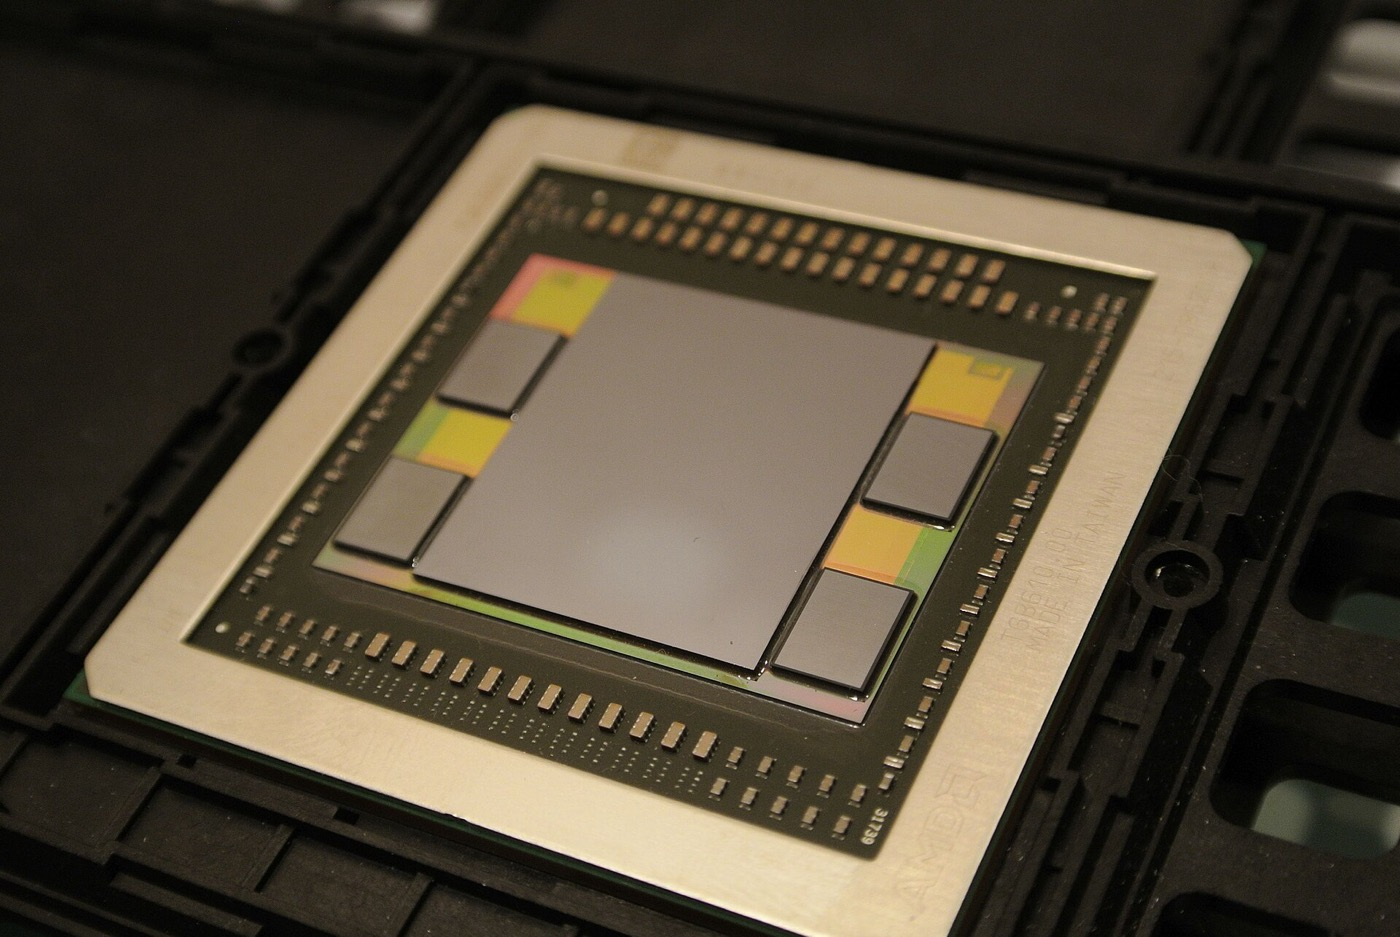
\includegraphics[width=\textwidth,height=1.7cm,keepaspectratio]{amd-fiji-hbm.jpg}\\[0.02cm]
      {\footnotesize\textcolor{midgray}{Four HBM stacks beside a GPU die}}
    \end{column}
  \end{columns}
  \mlsyscredit{Intensity and 140 GB: \S6.7.4; split: \S16.4. H100: 989 TFLOP/s dense FP16, 3.35 TB/s (MLSysIM). Photo: AMD Fiji package, C. Spille/pcgameshardware.de, CC BY-SA 4.0, Wikimedia Commons.}
  \note{[3.5 min] Worked example 4. The photo shows where the 3.35 TB/s comes from, stacks of high-bandwidth memory beside the processor (AMD's Fiji GPU of 2015; an H100 packages its HBM3 the same way). Step 1: decode at batch one with 16-bit weights does 2 FLOPs per 2-byte weight, 1 FLOP per byte (chapter 6.7.4). An H100 does 989 trillion FP16 FLOPs per second and reads 3.35 TB per second, so it needs 295 FLOPs per byte to keep its arithmetic busy. Decode sits 295 times below that line. ENGAGE: two minutes in pairs on tokens per second. Step 2: a 70-billion-parameter model in FP16 is 140 GB, more than one 80 GB H100 holds, so it is split across two; every byte is still read for every token, 70 GB on each GPU at the same time. Step 3: 70 GB divided by 3.35 TB per second is 21 milliseconds. Step 4: at most about 48 tokens per second, whatever the peak FLOP/s; the arithmetic takes well under a millisecond, and the KV cache only adds bytes. WARN: students reach for the 989 TFLOP/s and get thousands of tokens per second; ask which number the weights travel through. LINK, one line only: Lecture 13b shows how a server batches decode to share each weight read. FLEX: [CORE].}
\end{frame}

\begin{frame}{The KV cache keeps keys and values; each step reads them all}
  \centering
  \begin{tikzpicture}[font=\small]
    \foreach \x/\t/\c in {1.0/Queries/BlueLine, 3.8/Keys/RedLine, 5.2/Values/GreenLine}
      \node[font=\small\bfseries, text=\c] at (\x,2.65) {\t};
    \foreach \i/\w in {1/The, 2/cat, 3/sat, 4/on} {
      \node[text=darktext] at (2.4,2.6-0.55*\i) {\w};
      \only<1|handout:0>{\node[cell=1.2cm, fill=BlueLine!12] at (1.0,2.6-0.55*\i) {$q_{\i}$};}
      \only<2-|handout:1>{\node[cell=1.2cm, fill=vlightgray, text=lightgray] at (1.0,2.6-0.55*\i) {$q_{\i}$};
        \draw[RedLine, line width=1pt] (0.5,2.6-0.55*\i) -- (1.5,2.6-0.55*\i);}
      \node[cell=1.2cm, fill=RedLine!12] at (3.8,2.6-0.55*\i) {$k_{\i}$};
      \node[cell=1.2cm, fill=GreenLine!12] at (5.2,2.6-0.55*\i) {$v_{\i}$};}
    \only<1|handout:0>{
      \draw[VioletLine, line width=1.4pt, dashed, rounded corners=3pt] (3.05,2.33) rectangle (5.95,-0.13);
      \node[text=VioletLine, font=\small\bfseries, anchor=north] at (4.5,-0.2) {KV cache, one layer};}
    \only<2-|handout:1>{
      \node[text=midgray, font=\footnotesize, align=center, anchor=north] at (1.0,-0.45) {computed once,\\never read again};
      \node[text=darktext, font=\small\bfseries] at (2.4,-0.15) {the};
      \node[cell=1.2cm, fill=RedLine!35, draw=RedLine, line width=1.2pt] at (3.8,-0.15) {$k_5$};
      \node[cell=1.2cm, fill=GreenLine!35, draw=GreenLine, line width=1.2pt] at (5.2,-0.15) {$v_5$};
      \draw[VioletLine, line width=1.4pt, dashed, rounded corners=3pt] (3.05,2.33) rectangle (5.95,-0.68);
      \node[text=VioletLine, font=\small\bfseries, anchor=north] at (4.5,-0.75) {KV cache, one layer};
      \node[draw=BlueLine, fill=BlueLine!12, line width=1pt, minimum width=1.3cm, minimum height=0.6cm, align=center] (q) at (9.6,1.0) {$q_5$};
      \node[text=BlueLine, font=\footnotesize, align=center, anchor=north] at (9.6,0.55) {new query,\\used once};
      \foreach \i in {1,...,5} \draw[-{Stealth[length=2mm]}, line width=0.8pt, color=BlueLine] (q.west) -- (6.0,2.6-0.55*\i);
      \node[text=BlueLine, font=\footnotesize, align=center] at (7.75,2.65) {scores every $k$,\\mixes every $v$};}
  \end{tikzpicture}\\[0.25cm]
  \normalsize
  \only<1|handout:0>{Prefill computed $q$, $k$, and $v$ for each prompt token, in every layer.}%
  \only<2-|handout:1>{Each decode step appends one key and one value and reads every row.}
  \mlsyscredit{After Network Architectures, \S6.7.4 (Autoregressive decoding). Tokens: the prefill and decode example, \S6.7.2.}
  \note{[2 min] One layer of the decoder after the prompt ``The cat sat on''. Step 1: prefill computed a query, a key, and a value for every prompt token, as in the toy. The keys and values go into the KV cache, one such store per layer. Step 2: decode. The model emitted ``the'', and that token is now the input. Its key and value are appended as row 5. Its query, q5, scores every key in the cache and mixes every value, rows 1 to 5, to predict the next token. The old queries are crossed out, because an earlier token never attends to a later one, so no step reads q1 to q4 again, and q5 is discarded after this step too. ENGAGE: ``Why keep k and v instead of recomputing them?'' Expected: recomputing would rerun the whole prefix through every layer at every step. WARN: the cache is not optional bookkeeping; decode reads all of it at every step, so its bytes join the weights in the data term. FLEX: [CORE].}
\end{frame}

\begin{frame}{Each token GPT-2 XL keeps costs 307 KB of cache}
  \centering
  {\large KV cache per token $= 2 \times \text{layers} \times \text{key-value width} \times \text{bytes}$}\\[0.35cm]
  \uncover<2->{{\large $= 2 \times 48 \times 1{,}600 \times 2\ \text{B} =$ {\LARGE\textbf{\textcolor{mlsysaccent}{307.2 KB}}}}\\[0.3cm]}
  \uncover<3->{{\normalsize At its 1,024-token window: 314.6 MB for one sequence.}\\[0.35cm]}
  \uncover<4->{%
  {\normalsize key-value width $=$ key-value heads $\times$ head width\quad(GPT-2 XL: $25 \times 64 = 1{,}600$)}\\[0.1cm]
  \begin{tikzpicture}[font=\footnotesize]
    \foreach \i in {0,...,31} {
      \pgfmathtruncatemacro{\g}{\i/4}
      \fill[BlueLine] (0.19*\i,0.9) rectangle ++(0.13,0.3);
      \draw[midgray, line width=0.5pt] (0.19*\i+0.065,0.9) -- (0.76*\g+0.35,0.3);}
    \foreach \g in {0,...,7} \fill[RedLine] (0.76*\g+0.285,0) rectangle ++(0.13,0.3);
    \node[anchor=east, text=BlueLine, font=\footnotesize\bfseries] at (-0.15,1.05) {32 query heads};
    \node[anchor=east, text=RedLine, font=\footnotesize\bfseries] at (-0.15,0.15) {8 key-value heads};
    \node[anchor=west, text=darktext, align=left, font=\footnotesize] at (6.4,0.6)
      {\textbf{Llama 3.1 8B} (Meta):\\[0.02cm]
       \texttt{"dim": 4096,}\\
       \texttt{"n\_heads": 32,}\\
       \texttt{"n\_kv\_heads": 8,}\\[0.02cm]
       $8 \times 4{,}096/32 = 1{,}024$};
  \end{tikzpicture}}
  \mlsyscredit{Network Architectures, \S6.7.4 and Table 7 ($2Ld$ values per token); 314.6 MB: images/calcs.py. Llama 3.1 8B: github.com/meta-llama/llama-models, models/sku\_list.py (0e0b8c5), excerpted.}
  \note{[2.5 min] Step 1: the formula. A key and a value (the 2), for every layer, each as wide as the key-value width, in some number of bytes. Step 2: GPT-2 XL, 48 layers, width 1,600, FP16: 307.2 KB for every token a request keeps. Step 3: at its full 1,024-token window, one sequence holds 314.6 MB. Step 4: the key-value width is the number of key-value heads times the head width. GPT-2 XL gives each of its 25 heads of 64 its own keys and values, 1,600. Llama 3.1 8B has 32 query heads of 128, but each group of four shares one key-value head (the strip). The numbers come from Meta's own model list, with width 4,096, 32 heads, 8 key-value heads, so 4,096 over 32 is a head width of 128 and the key-value width is 8 times 128, 1,024, a quarter of the query width. This is grouped-query attention. ENGAGE: ``Which number in the formula did grouped heads change, and which would a narrower format change?'' Hold the answer for two slides. FLEX: [CORE].}
\end{frame}

\begin{frame}{The cache passes the weights near 10,000 tokens}
  \mlsysactivity{Predict}{1 min}
  \centering
  {\normalsize Predict: which comes first as context grows, the cache passing the weights,\\or one layer's scores (if stored) filling 80 GB?}\\[0.15cm]
  \mlsyssteps[width=0.92\textwidth,height=4.6cm,keepaspectratio]{context_memory_step}{3}
  \mlsyscredit{Slide redraw of the chapter's context-memory figure (\S6.7.4, figure 13): GPT-2 XL, FP16; KV 307.2 KB per token; scores for one layer, 25 heads.}
  \note{[2 min] [OPTIONAL] ENGAGE: thirty seconds, write a guess for each and which comes first. Three memories for one model as the context grows, log scales. Step 1: the weights, 3 GB in FP16, flat; they do not depend on context. Step 2: the KV cache for one request grows in a straight line, 307.2 KB per token, and passes the weights near 10,000 tokens. Step 3: one layer's scores, if stored, grow with the square and would fill an 80 GB accelerator near 40,000 tokens. Answer: the cache passes the weights first. The cache is the cost that cannot be tiled away, because decode needs it at every step. This plot uses GPT-2 XL's 25 heads (figure 13); the 240 GB example used Napkin Math 6.1's 12. WARN: the orange and red lines also cross, near 6,100 tokens; that crossing answers nothing here, so read the two dots. WARN: batching shares the weights across requests but not the caches; each request keeps its own. FLEX: if cut, say the cache passes the weights near 10,000 tokens.}
\end{frame}

\begin{frame}{In a real server, the KV cache takes over 30 percent of memory}
  \begin{columns}[c]
    \begin{column}{0.42\textwidth}
      \centering
      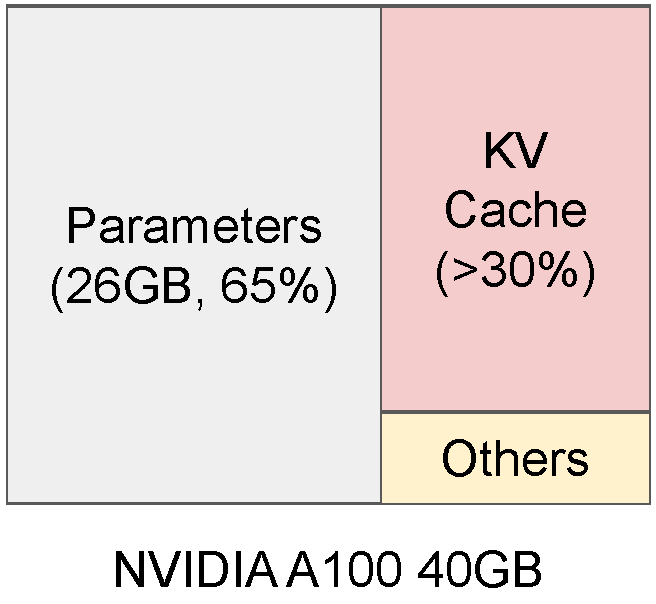
\includegraphics[width=\textwidth,height=4.6cm,keepaspectratio]{kwon2023_fig1_memory_layout.pdf}
    \end{column}
    \begin{column}{0.56\textwidth}
      \normalsize
      13B model, FP16, on one A100 40 GB\\[0.25cm]
      \uncover<2->{Per token: $2 \times 40 \times 5{,}120 \times 2$ B $=$ 0.82 MB\\[0.25cm]}
      \uncover<3->{One 2,048-token request: 1.68 GB\\[0.25cm]}
      \uncover<4->{{\large\textbf{\textcolor{mlsysaccent}{30\% of 40 GB: about 7 requests}}}}
    \end{column}
  \end{columns}
  \vspace{0.3cm}
  \centering
  \uncover<4->{\normalsize The weights stay at 26 GB; the KV cache space sets how many requests share one weight read.}
  \mlsyscredit{Figure: Kwon et al., ``Efficient Memory Management for LLM Serving with PagedAttention,'' SOSP 2023, Fig. 1 (left). OPT-13B shape: the paper, \S3. Values: images/calcs.py.}
  \note{[1.5 min] A measured layout from vLLM's authors. A 13-billion-parameter model is served on one A100 with 40 GB. The weights take 26 GB, 65 percent, and stay put; the KV cache takes more than 30 percent and comes and goes with the requests; activations are the small rest. Step 2: the paper's own arithmetic for OPT-13B is 2 times 40 layers times width 5,120 times 2 bytes, 0.82 MB per token (the paper writes 800 KB in binary units). Step 3: a full 2,048-token request keeps 1.68 GB. Step 4: so 30 percent of the card holds about seven such requests at once. ENGAGE: ``Halve the key-value width. What happens to the seven?'' Expected: about fourteen, which is the next slide. WARN: the paper's own fix, paging the cache to waste less of that 30 percent, is Lecture 13b; this lecture stops at the size. FLEX: [OPTIONAL] Give the 30 percent and seven requests aloud.}
\end{frame}

\begin{frame}{Sharing keys across heads cuts the cache fourfold or more}
  \centering
  \safeimg[width=0.95\textwidth,height=4.9cm,keepaspectratio]{kv_per_token.pdf}\\[0.1cm]
  \uncover<2->{\normalsize Llama 3.1 8B at its 128K window: 17.2 GB of cache, 16.1 GB of weights.}
  \mlsyscredit{Derived: $2 \times$ layers $\times$ key-value width $\times$ 2 B. Shapes: MLSysIM; Ainslie et al. 2023 (GQA); Shazeer 2019, Chowdhery et al. 2022 (PaLM). Window: Llama 3.1 model card.}
  \note{[1.5 min] KV cache per token in FP16 for five decoders, log scale. GPT-2 XL gives each of its 25 heads its own keys and values, 307 KB. Llama 2 7B does the same with 32 heads of 128: 524 KB. Llama 3.1 8B, grouped as on the strip, needs 131 KB, four times less (Llama 3 8B, used in Lectures 8 and 13b, has the same shape and a shorter window). Llama 2 70B shares 8 key-value heads among 64 query heads, so it needs 328 KB instead of 2.6 MB, eight times less. PaLM 540B uses one shared key-value head of width 256 (multi-query attention), for 121 KB. Step 2: Llama 3.1 8B holding its full 128K window keeps 17.2 GB of cache, more than its 16.1 GB of BF16 weights. WARN, the chapter's pitfall (section 6.10): a 7B model costs more than 14 GB to serve; at 2,048 tokens each request adds about 1 GB of cache. Earlier question: grouped heads change the key-value width; a narrower format changes the bytes. Landing line: ``Decode reads every weight for every token and keeps 2 L d values per token.'' FLEX: [OPTIONAL] If short, give the 4 times and 17.2 GB aloud.}
\end{frame}

% =============================================================================
% SECTION: EMBEDDINGS
% =============================================================================
\mlsysnote{[0.5 min] GPT-2 XL's token table was one embedding table. A recommender is built from hundreds. FLEX: [CORE].}
\mlsysdivider{Why is a recommender a memory machine?}{Network Architectures, \S6.8}
\section{Embeddings}

\begin{frame}{A recommender is mostly lookup tables around two small MLPs}
  \begin{columns}[c]
    \begin{column}{0.30\textwidth}
      \centering
      {\fontsize{40}{44}\selectfont\bfseries\textcolor{mlsysaccent}{79\%}}\\[0.3cm]
      {\small of AI inference cycles in Facebook's datacenters went to recommendation models}
    \end{column}
    \begin{column}{0.68\textwidth}
      \centering
      \uncover<2->{%
      \begin{tikzpicture}[font=\footnotesize]
        \node[blk=midgray, minimum width=2.3cm, minimum height=0.6cm, font=\footnotesize] (df) at (0,0) {Dense features};
        \node[blk=OrangeLine, minimum width=2.3cm, minimum height=0.6cm, font=\footnotesize] (bm) at (0,1.3) {Bottom MLP};
        \node[blk=midgray, minimum width=3.6cm, minimum height=0.6cm, font=\footnotesize] (ids) at (4.4,0) {Categorical IDs};
        \foreach \x/\y in {3.2/1.55, 4.4/1.15, 5.6/1.75} {
          \node[draw=BlueLine, fill=BlueL, line width=1pt, minimum width=0.8cm, minimum height=1.2cm] at (\x,1.4) {};
          \fill[BlueLine] (\x-0.4,\y-0.07) rectangle (\x+0.4,\y+0.07);}
        \node[font=\footnotesize, text=BlueLine, align=left, anchor=west] at (6.15,1.4) {\textbf{Embedding}\\\textbf{tables}};
        \node[blk=VioletLine, minimum width=7.6cm, minimum height=0.6cm, font=\footnotesize] (int) at (2.7,2.75) {Interaction (pairwise dot products)};
        \node[blk=OrangeLine, minimum width=3.6cm, minimum height=0.6cm, font=\footnotesize] (tm) at (2.7,3.75) {Top MLP $\rightarrow$ click probability};
        \draw[arr] (df) -- (bm); \draw[arr] (bm) -- (bm |- int.south);
        \foreach \x in {3.2,4.4,5.6} {\draw[arr] (\x,0.3) -- (\x,0.8); \draw[arr] (\x,2.0) -- (\x,2.45);}
        \draw[arr] (int) -- (tm);
      \end{tikzpicture}}
    \end{column}
  \end{columns}
  \vspace{0.3cm}
  \centering
  \uncover<3->{\normalsize Callback: GPT-2 XL's token table, 80M weights, is one such table.}
  \mlsyscredit{Share: Gupta et al., HPCA 2020. Pipeline after the chapter's DLRM figure (\S6.8.2, figure 14; Naumov et al. 2019).}
  \note{[2 min] Step 1: the number. Facebook reported that recommendation models used 79 percent of the AI inference cycles in its datacenters (Gupta et al. 2020). Step 2: DLRM, the recommendation lighthouse, in four stages. Dense features such as age or time of day go through a bottom MLP of ordinary matrix multiplies. Categorical IDs (user, item, items recently viewed) each select one learned row from an embedding table, the dark stripes. An interaction layer takes dot products among all the pieces, and a top MLP predicts the click. Step 3: the token table from GPT-2 XL had exactly this structure, one row per token. ENGAGE: ``Which stage does the arithmetic, and which stage holds the bytes?'' Expected: the MLPs and interaction do the arithmetic; the tables hold the bytes. FLEX: [CORE].}
\end{frame}

\begin{frame}{A request gathers scattered rows, and their home sets the rate}
  \begin{columns}[c]
    \begin{column}{0.62\textwidth}
      \centering
      \begin{tikzpicture}[font=\footnotesize]
        \draw[BlueLine, line width=1pt, rounded corners=3pt, fill=BlueL!40] (0,0) rectangle (8.6,2.25);
        \node[anchor=south west, text=BlueLine, font=\footnotesize\bfseries] at (0.1,0.02) {HBM: 26 tables, one per feature};
        \foreach \x/\y in {0.6/1.6, 1.6/1.0, 2.6/1.85, 3.6/1.3, 6.2/0.9, 7.2/1.7} {
          \draw[BlueLine, fill=white, line width=0.8pt] (\x-0.3,0.5) rectangle (\x+0.3,2.1);
          \fill[OrangeLine] (\x-0.3,\y-0.07) rectangle (\x+0.3,\y+0.07);}
        \node[text=BlueLine, font=\large\bfseries] at (4.9,1.3) {$\cdots$};
        \uncover<2->{
          \foreach \x in {0.6,1.6,2.6,3.6,6.2,7.2} {\draw[arr, color=OrangeLine] (\x,2.15) -- (\x,2.75);
            \fill[OrangeLine] (\x-0.3,2.82) rectangle (\x+0.3,2.97);}
          \node[text=OrangeLine, font=\footnotesize\bfseries] at (4.3,3.35) {26 rows $\times$ 512 B $=$ 13.3 KB copied, no arithmetic};}
        \uncover<3->{
          \node[blk=VioletLine, minimum width=8.6cm, minimum height=0.9cm, font=\footnotesize] at (4.3,4.55)
            {Interaction of 27 vectors: 351 dot products, 44,928 MACs\\about 7 FLOP per gathered byte};
          \draw[arr] (4.3,3.6) -- (4.3,4.05);}
      \end{tikzpicture}
    \end{column}
    \begin{column}{0.36\textwidth}
      \centering
      \uncover<4->{\safeimg[width=\textwidth,height=5.2cm,keepaspectratio]{recsys_rate.pdf}}
    \end{column}
  \end{columns}
  \mlsyscredit{Illustrative request: 26 categorical features as in Criteo (Naumov et al. 2019); 128-wide FP32 rows, 512 B (\S6.8.3). Bounds derived from MLSysIM H100 (HBM, PCIe Gen5 x16).}
  \note{[2.5 min] [OPTIONAL] An illustrative request is shaped like the Criteo benchmark DLRM was published on, with 26 categorical features, one 128-wide FP32 row each, 512 bytes per row. Step 1: the tables live in HBM, the accelerator's memory; each feature's ID lights one row, at an address that depends on the data, so the next address cannot be predicted. Step 2: the gather copies the 26 rows, 13.3 KB, with no arithmetic at all. Step 3: the interaction layer takes dot products among 27 vectors (the 26 rows and the bottom MLP's output), 351 pairs of 128, 44,928 multiply-adds, about 7 FLOPs per byte gathered, far below the H100's 295. Step 4: so the bytes set the rate. If every row streamed at HBM's 3.35 TB/s, one accelerator could feed at most 252 million such requests per second; if the tables sat in host memory across PCIe at 64 GB/s, 4.8 million, 52 times fewer. WARN: these are upper bounds. Scattered 512-byte reads reach less than either peak, and popular rows stay in cache while the long tail goes to DRAM. ENGAGE: ``What decides which of these two bars you get?'' Expected: whether the tables fit in HBM, the next slide. FLEX: if cut, go to the capacity estimate.}
\end{frame}

\begin{frame}[fragile]{Estimate: does one table fit an 80 GB accelerator?}
  \mlsysactivity{Estimate}{2.5 min}
  \begin{columns}[T]
    \begin{column}{0.36\textwidth}
      \begin{mlsyscard}{mlsysaccent}
        \textbf{Given}\\[0.1cm]
        100 million items\\
        128 numbers per row\\
        FP32 (4 bytes)\\
        One A100: 80 GB
      \end{mlsyscard}
    \end{column}
    \begin{column}{0.60\textwidth}
      \normalsize
      \uncover<2->{$10^8 \times 128 \times 4$ bytes $=$ {\Large\textbf{\textcolor{mlsysaccent}{51.2 GB}}}\\[0.15cm]}
      \uncover<3->{51.2 / 80 $=$ 64\% of the device, for one feature\\[0.15cm]}
      \uncover<4->{Add a user table of the same size: 102.4 GB.\\[0.15cm]}
      \uncover<5->{A billion users: 512 GB for that table alone.}
    \end{column}
  \end{columns}
  \vspace{0.05cm}
  {\footnotesize\textbf{DLRM builds each table in one line}, \texttt{n} rows of width \texttt{m}:}
\begin{semiverbatim}\footnotesize
EE = nn.EmbeddingBag(n, m, mode="sum", sparse=True)
\end{semiverbatim}
  \mlsyscredit{Network Architectures, Napkin Math 6.2 and \S6.8.2. Code: dlrm\_s\_pytorch.py, DLRM\_Net.create\_emb (github.com/facebookresearch/dlrm, commit 9bc1bc3, MIT).}
  \note{[2.5 min] Worked example 5. The code line at the bottom is how Facebook's open DLRM creates every table, as a PyTorch EmbeddingBag of n rows, each m numbers wide, that sums the rows a request selects. Today's n is 100 million and m is 128. ENGAGE: ninety seconds in pairs. Step 2: 100 million rows times 128 numbers times 4 bytes, 51.2 GB. Step 3: 64 percent of an 80 GB A100, for one categorical feature, before any activations or the MLPs. Step 4: a user table of the same size brings the total to 102.4 GB, which does not fit. Step 5: at a billion users, 128 wide, the user table alone is 512 GB. Students who get 51.2 MB dropped a factor of 1,000. WARN: FLOP counts do not answer this question; the question is where the table can live. FLEX: [CORE].}
\end{frame}

\begin{frame}{Capacity decides where the tables live before speed matters}
  \begin{columns}[T]
    \begin{column}{0.54\textwidth}
      \centering
      \safeimg[width=\textwidth,height=3.3cm,keepaspectratio]{capacity.pdf}\\[0.3cm]
      \uncover<2->{%
      \begin{tabular}{@{}ccc@{}}
        \textbf{\textcolor{BlueLine}{Shrink}} & \textbf{\textcolor{BlueLine}{Move}} & \textbf{\textcolor{BlueLine}{Partition}} \\
        {\footnotesize hash, compress} & {\footnotesize host DRAM, PCIe} & {\footnotesize across devices}
      \end{tabular}}
    \end{column}
    \begin{column}{0.42\textwidth}
      \centering
      \uncover<3->{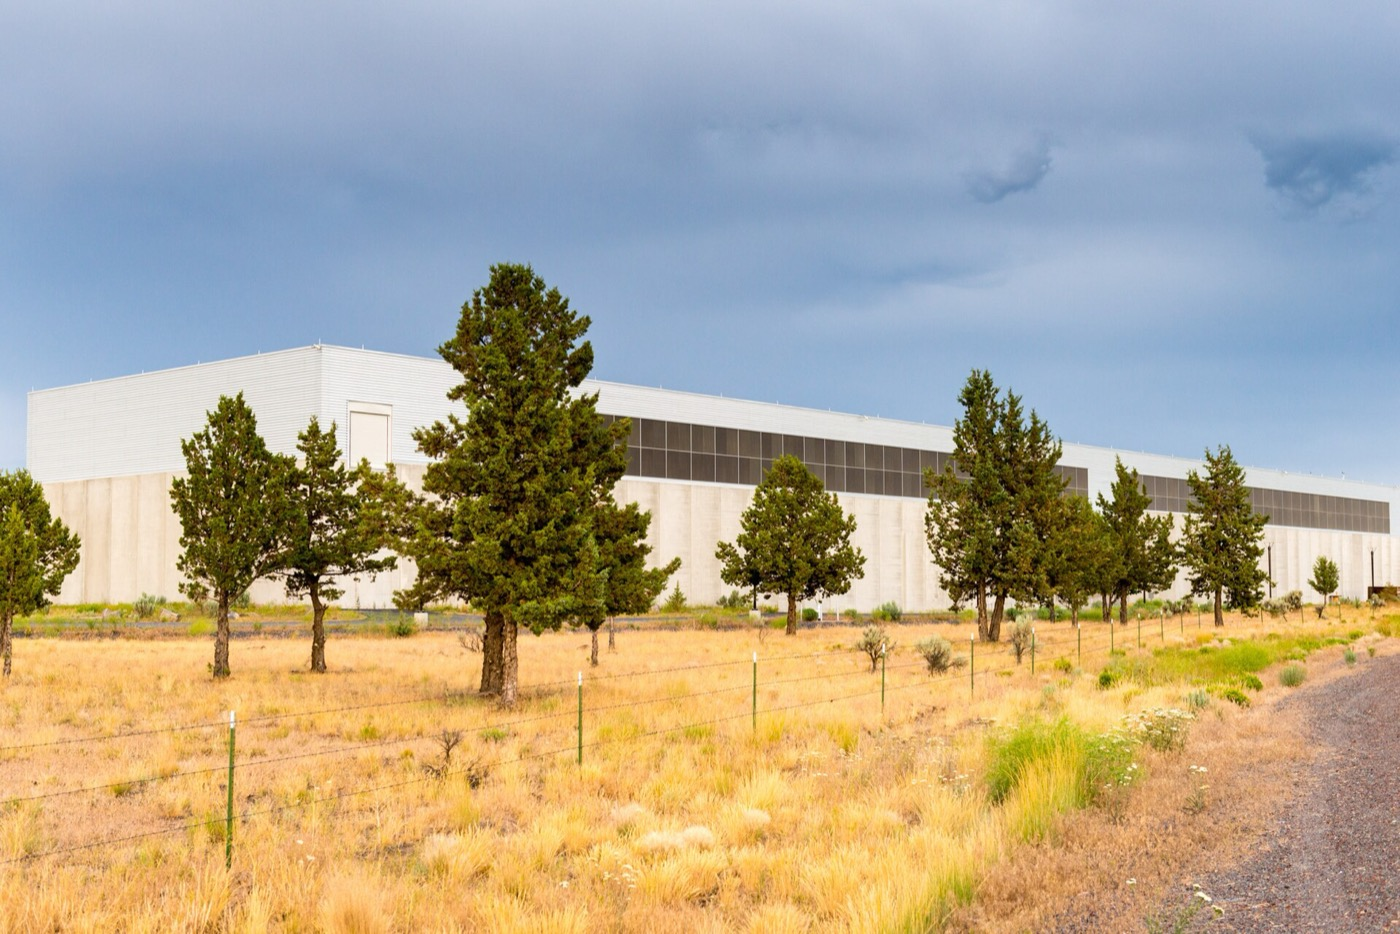
\includegraphics[width=\textwidth,height=3.4cm,keepaspectratio]{facebook-prineville.jpg}\\[0.05cm]
      {\footnotesize\textcolor{midgray}{Facebook's datacenter, Prineville, Oregon}}\\[0.1cm]
      {\small ``train very large DLRMs with up to 12 Trillion parameters''}}
    \end{column}
  \end{columns}
  \mlsyscredit{Network Architectures, Napkin Math 6.2 and \S6.8.3. Quote: Mudigere et al., Facebook, arXiv 2104.05158 (ISCA 2022). Photo: Gary Halvorson, Oregon State Archives, 8 July 2014, CC BY 4.0, Wikimedia Commons.}
  \note{[2 min] Step 1: the estimate as bars. One table fits at 64 percent; two cross the 80 GB line. Step 2: the three ways out, each with its price. Shrink the tables (hashing, compression, pruning), at the risk of losing rare users and items. Move them to host memory, where every lookup crosses PCIe, the 52 times lower bar on the previous slide. Partition them across accelerators. Step 3: partitioning makes each request need rows held by every device, an all-to-all exchange in which every device sends to every other. Production systems do this at the scale of a building. The photo is Facebook's Prineville datacenter, and a Facebook team reported training DLRMs with up to 12 trillion parameters, 48 TB of FP32 weights. In iron-law terms, capacity is a check that comes before both terms, because it decides which bandwidth the data term pays. Partitioning is left to the reading (section 6.8.3). Landing line for the segment: ``A recommender's bytes are scattered rows, so where its tables live comes first.'' FLEX: [CORE].}
\end{frame}

% =============================================================================
% SECTION: CHOOSING
% =============================================================================
\mlsysnote{[0.5 min] All five lighthouses are now on the table. Put them side by side. FLEX: [CORE].}
\mlsysdivider{With all five families on the table, what limits each one?}{Network Architectures, \S6.9 and \S6.10}
\section{Choosing}

\begin{frame}{Your turn: what limits each lighthouse?}
  \mlsysactivity{Diagnose}{2 min}
  \centering\footnotesize
  \renewcommand{\arraystretch}{1.3}
  \begin{tabular}{@{}l l r r l@{}}
    \toprule
    \textbf{Lighthouse} & \textbf{Family} & \textbf{\shortstack[r]{FLOP/byte\\(FP32)}} & \textbf{Training state} & \textbf{Binding limit} \\
    \midrule
    \textcolor{midgray}{ResNet-50} & \textcolor{midgray}{CNN} & \textcolor{midgray}{80.1} & 409.6 MB & \textcolor{midgray}{Compute} \\
    \textcolor{midgray}{MobileNetV2} & \textcolor{midgray}{depthwise CNN} & \textcolor{midgray}{42.8} & 56.1 MB & \textcolor{midgray}{Compute (phone latency)} \\
    \textcolor{midgray}{KWS (DS-CNN)} & \textcolor{midgray}{depthwise CNN} & \textcolor{midgray}{25} & 3.2 MB & \textcolor{midgray}{Power, milliwatts} \\
    \midrule
    GPT-2 XL & transformer & 0.50 & 24 GB & \uncover<2->{\textbf{\textcolor{BlueLine}{Decode bandwidth}}} \\
    DLRM & embeddings + MLPs & n/a & \alert<3->{400 GB} & \uncover<3->{\textbf{\textcolor{VioletLine}{Capacity}}} \\
    \bottomrule
  \end{tabular}\\[0.3cm]
  {\normalsize Select by workload profile. Gray rows: Part 1's answers. Diagnose the last two;}\\
  {\normalsize then, which models could train on one 80 GB accelerator?}
  \mlsyscredit{Network Architectures, Tables 8 and 10. Intensity: FLOPs over FP32 weight bytes (weight-only proxy). Training state: 16 B per parameter.}
  \note{[3.5 min] The chapter's comparison. The gray rows are Part 1's diagnosis; only their training state is new. Explain the number columns first. FLOP per byte is the chapter's weight-only proxy with FP32 weights (so decode shows 0.50 against the FP16 slide's 1.0); do not set it against the H100's FP16 ridge of 295. Training state is 16 bytes per parameter, the FP32 weight, its gradient, and two optimizer moments. ENGAGE: ninety seconds in pairs on the two new rows and the question, then reveal (steps 2 and 3), asking one pair per row for its reasoning. GPT-2 XL: decode reads every weight per token, so bandwidth binds, plus 307.2 KB of cache per token. At GPT-2 XL's size one decode step reads its weights in about 0.9 ms, a few times shorter than the time to launch the step's many small kernels, so launch overhead competes with bandwidth; Lecture 7 counts those kernels. DLRM: 100 GB of tables before anything runs. The question: all but DLRM, whose 400 GB of training state does not fit. WARN: the chapter's fallacy that complex architectures always win; vision transformers matched CNNs on ImageNet only with far larger pretraining. LINK: Part 1's Netflix Prize scored only the accuracy column. FLEX: [CORE].}
\end{frame}

\begin{frame}{A million-token request is a memory budget first}
  \centering
  \mlsyssteps[width=0.95\textwidth,height=3.9cm,keepaspectratio]{million_request_step}{3}\\[0.2cm]
  \uncover<3->{\normalsize Attention arithmetic: about $5 \times 10^{17}$ FLOP per prompt, nearly 9 minutes of H100 peak.\\[0.15cm]
  \textbf{\textcolor{mlsysaccent}{Hook answer: B.}} Score work 250,000$\times$; memory 500$\times$.}
  \mlsyscredit{Illustrative: a model of Llama 3.1 8B's shape (its card states 128K) at 1M tokens. Derived from MLSysIM Llama3\_8B and H100.}
  \note{[2.5 min] Return to the hook and price one full request at the largest window on the plot, using a model of Llama 3.1 8B's shape; the shape is real, the million-token use is illustrative, since that model's card states 128K. Step 1: its weights in BF16, a 16-bit format, 16.1 GB, under the 80 GB line. Step 2: the KV cache at 131,072 bytes per token, times a million tokens, 131 GB, so the request alone does not fit one device. Step 3: the scores, if stored, would be 2 TB for one head of one layer, so no kernel stores them (Lecture 8b). The arithmetic remains, two attention products of S squared times 4,096 over 32 layers, about 5 times 10 to the 17th FLOPs, nearly 9 minutes of an H100's peak for one prompt, about half that with the causal mask skipping the masked half. Answer to the hook: B. Score work grows with the square of the window, 250,000 times; the memory a request keeps grows with the window, 500 times. Say the closing sentence: ``A 1M-token window first has to fit in memory.'' FLEX: [CORE].}
\end{frame}

\begin{frame}{Takeaways}
  \normalsize
  \begin{itemize}\setlength{\itemsep}{0.3cm}
    \item Attention scores every pair: score work grows with $S^2$.
    \item A block holds $12d^2$ weights; attention's work dominates only past $6d$ tokens.
    \item Decode reads every weight per token and keeps $2Ld$ values per token.
    \item A recommender's bytes are scattered rows; where its tables live comes first.
  \end{itemize}
  \note{[1.5 min] One line per segment. Ask students to circle the one they could not have explained an hour ago and to write the number that goes with it (S squared; 9,600; 307.2 KB; 51.2 GB). FLEX: [CORE].}
\end{frame}

\begin{frame}{Open questions}
  \begin{columns}[c]
    \begin{column}{0.60\textwidth}
      \normalsize
      \begin{itemize}\setlength{\itemsep}{0.35cm}
        \item A longer window costs memory in proportion and work in square. Is it worth it if models use long contexts less well?
        \item Should a context window be priced by the token?
        \item If a recommender's main operation is a copy, should its hardware look more like a memory system?
      \end{itemize}
    \end{column}
    \begin{column}{0.38\textwidth}
      \centering
      \safeimg[width=\textwidth,height=4.2cm,keepaspectratio]{fiction_livebench.pdf}\\[0.05cm]
      {\footnotesize\textcolor{midgray}{DeepSeek-R1-0528, Fiction.LiveBench}}
    \end{column}
  \end{columns}
  \mlsyscredit{Fiction.LiveBench scores via the Epoch AI Benchmarking Hub (CC BY 4.0), MLSysIM literature series.}
  \note{[1.5 min] No single answer. The first: on Fiction.LiveBench, a test of understanding a story placed in context, DeepSeek-R1-0528 scores 0.917 with 400 tokens of story and 0.583 with 60,000; longer windows cost more and may be used less well. The second: providers price per token, while score work grows faster than the tokens. The third: the copy-dominated recommender against hardware built around matrix units. Ask students to write one sentence on one of them. FLEX: [OPTIONAL].}
\end{frame}

\begin{frame}{Read and explore}
  \small
  \begin{itemize}\setlength{\itemsep}{0.05cm}
    \item \textbf{Read:} Network Architectures, \S6.6 to \S6.10, and the self-checks in \S6.6 to \S6.8.
    \item \textbf{Practice:} the TinyTorch attention module.
    \item Alammar, ``The Illustrated Transformer,'' 2018 (jalammar.github.io).
    \item Vaswani et al., ``Attention Is All You Need,'' NeurIPS 2017.
    \item Shazeer, ``Fast Transformer Decoding: One Write-Head is All You Need,'' 2019.
    \item Naumov et al., ``Deep Learning Recommendation Model for Personalization and Recommendation Systems,'' 2019.
    \item Gupta et al., ``The Architectural Implications of Facebook's DNN-based Personalized Recommendation,'' HPCA 2020.
  \end{itemize}
  \note{[1 min] The chapter first; \S6.7.4 covers prefill, decode, and the cache, and \S6.9 collects the counting rules for all five families in one table. Alammar draws queries, keys, values, and heads step by step, as the toy did. Vaswani et al. is the transformer; Shazeer introduced multi-query attention, the cache-shrinking idea on the PaLM bar; Naumov et al. and Gupta et al. are the recommender and its systems costs. FLEX: [OPTIONAL] Replace a paper with your own lab or TinyTorch module.}
\end{frame}

\begin{frame}[c]
  \centering
  {\small\textcolor{lightgray}{NEXT LECTURE \textbar{} ML FRAMEWORKS}}\\[0.5cm]
  {\LARGE\bfseries How does Python code become\\kernels on the hardware?}
  \note{[0.5 min] Two lectures fixed what work each architecture must do and what it commits the machine to. Next time: who decides when that work runs, how its gradients are computed, and which device runs it. Ask students to read ML Frameworks before then. FLEX: [CORE].}
\end{frame}

\end{document}
